\documentclass[border = 1cm, preview, varwidth=\maxdimen]{standalone}

\usepackage{xeCJK}

% mathematics
\usepackage{amsmath}

% tikz
\usepackage{tikz}
\usepackage{ifthen}
\usetikzlibrary{arrows}
\usetikzlibrary{automata}
\usetikzlibrary{positioning}
\tikzset{
  ->,
  >=stealth',
  node distance = 1.5cm,
}

\begin{document}
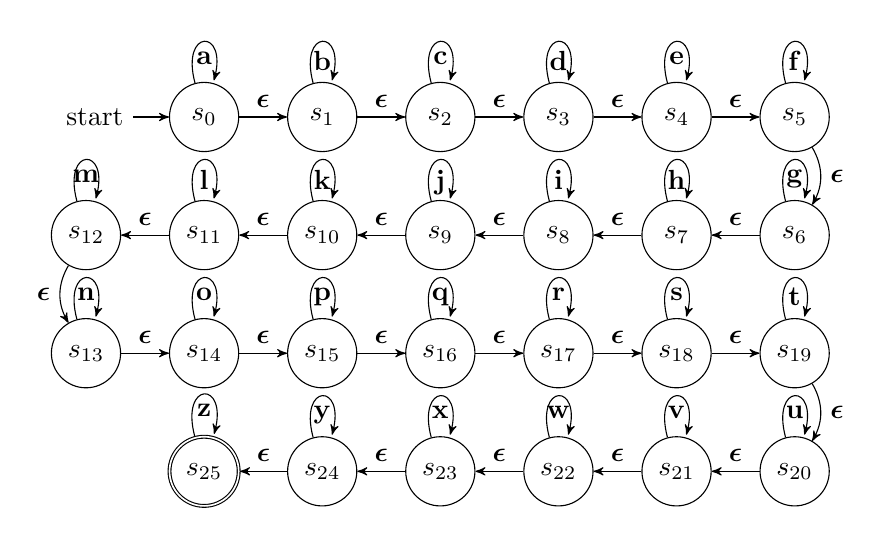
\begin{tikzpicture}
  % nodes
  \node [state, initial] (s0) {$s_0$};
  \foreach \curr in {1, ..., 24} {
    \pgfmathtruncatemacro \prev { \curr - 1 };
    \pgfmathtruncatemacro \isrowlast { mod(\curr, 7) - 6 };
    \ifthenelse{\isrowlast = 0}
      {\node [state, below of = s\prev] (s\curr) {$s_{\curr}$};}
      {
        \pgfmathtruncatemacro \isevenrow { mod(\curr, 14) - 6 };
        \ifthenelse {\isevenrow < 0}
          {\node [state, right of = s\prev] (s\curr) {$s_{\curr}$};}
          {\node [state, left of = s\prev] (s\curr) {$s_{\curr}$};}
      }
  }
  \node [state, accepting, left of = s24] (s25) {$s_{25}$};
  % paths
  \foreach \char [count = \index] in {a, ..., z} {
    \pgfmathtruncatemacro \identity { \index - 1 };
    \draw (s\identity) edge [loop above, below] node {\textbf\char} (s\identity);
  }
  \foreach \curr in {1, ..., 5, 7, 8, ..., 12, 14, 15, ..., 19, 21, 22, ..., 25} {
    \pgfmathtruncatemacro \prev { \curr - 1 };
    \draw (s\prev) edge [above] node {$\boldsymbol\epsilon$} (s\curr);
  }
  \draw (s5) edge [right, bend left] node {$\boldsymbol\epsilon$} (s6);
  \draw (s12) edge [left, bend right] node {$\boldsymbol\epsilon$} (s13);
  \draw (s19) edge [right, bend left] node {$\boldsymbol\epsilon$} (s20);
\end{tikzpicture}
\end{document}
